\section[Lecture 2: Lagrangian Mechanics, Euler-Lagrange Equations, and Hamiltonians]
 {\texorpdfstring{Lecture 2:\\ Lagrangian Mechanics, Euler-Lagrange Equations, and Hamiltonians}
  {Lecture 2: Lagrangian Mechanics, Euler-Lagrange Equations, and Hamiltonians}}

\subsection{Conservative Forces and the Lagrangian}

A \textbf{conservative force} is one for which the work done along any closed path is zero. Formally, for a particle labeled by $\alpha$, this means:
\begin{equation}
    \oint \mathbf{F}_\alpha \cdot d\mathbf{r}_\alpha = 0.
\end{equation}
As a consequence, a conservative force can be expressed as the negative gradient of a potential energy function $V$:
\begin{equation}
    \mathbf{F}_\alpha = -\nabla_\alpha V(\mathbf{r}_1,\, \dots,\, \mathbf{r}_\alpha).
\end{equation}

Since the particle positions $\mathbf{r}_\alpha$ depend on the generalized coordinates $q_i$, the potential energy may be written as
\begin{equation}
    V(\mathbf{r}_\alpha) = V(q_i, t).
\end{equation}
Using the chain rule, one finds:
\begin{equation}
    \frac{\partial V}{\partial q_i} = \sum_\alpha \frac{\partial V}{\partial \mathbf{r}_\alpha} \cdot \frac{\partial \mathbf{r}_\alpha}{\partial q_i} = -\sum_\alpha \mathbf{F}_\alpha \cdot \frac{\partial \mathbf{r}_\alpha}{\partial q_i} = -Q_i,
\end{equation}
where $Q_i$ is the generalized force associated with the coordinate $q_i$.

For conservative systems, the work done is path independent. Moreover, if the kinetic energy is expressed as $T(q_i, \dot{q}_i, t)$, then—as shown in Lecture 1—the generalized force takes the form:
\begin{equation}
    Q_i = \frac{d}{dt}\left(\frac{\partial T}{\partial \dot{q}_i}\right) - \frac{\partial T}{\partial q_i}.
\end{equation}

\subsubsection{The Lagrangian Function and the Euler-Lagrange Equations}

Define the \textbf{Lagrangian} as:
\begin{equation}
    L(q_i, \dot{q}_i, t) = T(q_i, \dot{q}_i, t) - V(q_i, t).
\end{equation}
Substituting the expression for $F_i$, the equation of motion becomes
\begin{equation}
    \frac{d}{dt}\left(\frac{\partial T}{\partial \dot{q}_i}\right) - \frac{\partial T}{\partial q_i} + \frac{\partial V}{\partial q_i} = 0.
\end{equation}
Because the potential energy $V$ is independent of $\dot{q}_i$, the above expression can be neatly recast into the \textbf{Euler-Lagrange equations}:
\begin{equation}
    \frac{d}{dt}\left(\frac{\partial L}{\partial \dot{q}_i}\right) - \frac{\partial L}{\partial q_i} = 0.
\end{equation}
These $N$ second-order differential equations (one for each degree of freedom) serve as the foundation for analyzing the dynamics of conservative systems.

\subsubsection{A Worked Example: The Simple Pendulum}

\begin{figure}[ht]
    \centering
    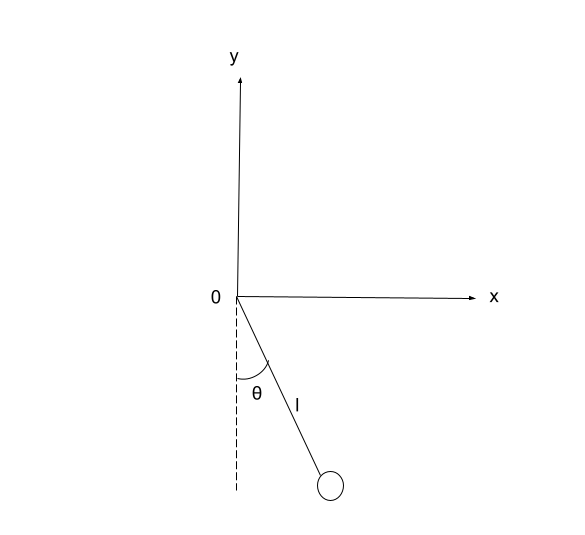
\includegraphics[width=0.3\textwidth]{images/2-1-1.png}
    \caption{Schematic of a Simple Pendulum}
    \label{fig:2-1-1}
\end{figure}

Consider a simple pendulum of mass $m$ and length $l$ (see Figure~\ref{fig:2-1-1}). The position of the pendulum bob in Cartesian coordinates is given by:
\begin{align}
    x & = l\sin\theta,  \\
    y & = -l\cos\theta.
\end{align}
Taking time derivatives yields:
\begin{align}
    \dot{x} & = l\cos\theta\,\dot{\theta}, \\
    \dot{y} & = l\sin\theta\,\dot{\theta}.
\end{align}
Thus, the kinetic energy is:
\begin{equation}
    T = \frac{1}{2} m (\dot{x}^2 + \dot{y}^2) = \frac{1}{2}ml^2\dot{\theta}^2.
\end{equation}
Choosing the gravitational potential energy as
\begin{equation}
    V = -mgl\cos\theta,
\end{equation}
the Lagrangian becomes:
\begin{equation}
    L = T - V = \frac{1}{2}ml^2\dot{\theta}^2 + mgl\cos\theta.
\end{equation}
Applying the Euler-Lagrange equation for $\theta$, we have:
\begin{equation}
    \frac{d}{dt}\left(\frac{\partial L}{\partial\dot{\theta}}\right) - \frac{\partial L}{\partial\theta} = \frac{d}{dt}(ml^2\dot{\theta}) + mgl\sin\theta = 0,
\end{equation}
which simplifies to:
\begin{equation}
    ml^2\ddot{\theta} + mgl\sin\theta = 0.
\end{equation}
This is the familiar equation of motion for a simple pendulum.

In summary, given a system with $M$ particles and $N$ degrees of freedom, the following
steps should be followed to determine the equations of motion using Lagrangian Mechanics:

\begin{enumerate}
    \item Identify the generalized coordinates $q_i$ that specify the system's
          configuration, and express the position vectors of the particles as
          $\mathbf{r}_\alpha=\mathbf{r}_\alpha(q_i, t)$, where $\alpha = 1, 2, \dots, M$ and
          $i = 1, 2, \dots, N$.
    \item Calculate the kinetic energy
          $T = \sum_\alpha \frac{1}{2} m_\alpha \dot{\mathbf{r}}_\alpha \cdot \dot{\mathbf{r}}_\alpha$
          as a function of $q_i$ and $\dot{q}_i$.
    \item Compute the potential energy $V = V(\mathbf{r}_\alpha) = V(q_i, t)$.
    \item Construct the Lagrangian $L = T - V$.
    \item Apply the Euler-Lagrange equations:
          $\frac{d}{dt} \left(\frac{\partial L}{\partial \dot{q}_i}\right) - \frac{\partial L}{\partial q_i} = 0$.
\end{enumerate}

\subsection{Hamiltonian Mechanics}

While the Lagrangian formulation provides a powerful method for deriving the equations of motion, the Hamiltonian formulation offers an alternative perspective—often advantageous in areas such as canonical transformations, quantum mechanics, and statistical mechanics.

\subsubsection{Definition of the Hamiltonian}

For a system described by generalized coordinates $q_i$ and velocities $\dot{q}_i$, the \textbf{Hamiltonian} is defined as the Legendre transform of the Lagrangian:
\begin{equation}
    H(q_i, p_i, t) = \sum_i \dot{q}_i\, p_i - L(q_i, \dot{q}_i, t),
\end{equation}
where the \textbf{generalized momentum} conjugate to $q_i$ is given by:
\begin{equation}
    p_i = \frac{\partial L}{\partial \dot{q}_i}.
\end{equation}

\subsubsection{Conservation of Energy and Time-Translation Symmetry}

To understand the time evolution of $H$, consider its total time derivative:
\begin{align}
    \frac{dH}{dt} & = \sum_i\left(\ddot{q}_i\,\frac{\partial L}{\partial \dot{q}_i} + \dot{q}_i\,\frac{d}{dt}\left(\frac{\partial L}{\partial \dot{q}_i}\right)\right) - \frac{dL}{dt} \nonumber \\[1mm]
                  & = \sum_i\left(\ddot{q}_i\,\frac{\partial L}{\partial \dot{q}_i} + \dot{q}_i\,\frac{d}{dt}\left(\frac{\partial L}{\partial \dot{q}_i}\right)\right) - \left(\sum_i\left(\frac{\partial L}{\partial q_i} \dot{q_i} + \frac{\partial L}{\partial \dot{q_i}} \ddot{q_i}\right)\right) - \frac{\partial L}{\partial t}
\end{align}
Using the Euler-Lagrange equations, the bracketed term vanishes, leaving:
\begin{equation}
    \frac{dH}{dt} = -\frac{\partial L}{\partial t}.
\end{equation}
Thus, if the Lagrangian is \emph{time-independent} (i.e., $\partial L/\partial t = 0$), then:
\begin{equation}
    \frac{dH}{dt} = 0,
\end{equation}
implying that the Hamiltonian is conserved. For many systems, especially when constraints are time-independent and $V$ depends only on coordinates, the Hamiltonian corresponds to the total energy:
\begin{equation}
    H = T + V.
\end{equation}

\subsubsection{Another Example: Particle Moving in a Circle}

Consider a particle of mass $m$ moving along a circle of fixed radius $R$. Using the angular coordinate $\theta$, the position is parameterized as:
\begin{align}
    x & = R\cos\theta, \\
    y & = R\sin\theta.
\end{align}
The kinetic energy is:
\begin{equation}
    T = \frac{1}{2}mR^2\dot{\theta}^2.
\end{equation}
Since the motion is confined to a circle, there is no potential energy (or it is constant, and can be set to zero):
\begin{equation}
    V = 0.
\end{equation}
Thus, the Lagrangian is:
\begin{equation}
    L = \frac{1}{2}mR^2\dot{\theta}^2.
\end{equation}
The generalized momentum is:
\begin{equation}
    p_\theta = \frac{\partial L}{\partial \dot{\theta}} = mR^2\dot{\theta},
\end{equation}
which is recognized as the \emph{angular momentum}. The Hamiltonian then is:
\begin{equation}
    H = \dot{\theta}\,p_\theta - L = mR^2\dot{\theta}^2 - \frac{1}{2}mR^2\dot{\theta}^2 = \frac{1}{2}mR^2\dot{\theta}^2 = T.
\end{equation}
Since $L$ is independent of $\theta$, the angular momentum $p_\theta$ is conserved. This result reflects the underlying rotational symmetry of the system.

\subsection{Noether's Theorem and Symmetries}

An elegant feature of Lagrangian mechanics is its ability to relate continuous symmetries to conservation laws through \textbf{Noether's Theorem}. In essence:
\begin{quotation}
    \emph{Every continuous symmetry of the action of a physical system has a corresponding conservation law.}
\end{quotation}
For example:
\begin{itemize}
    \item \textbf{Time-translation symmetry} (i.e., $\partial L/\partial t = 0$) implies conservation of energy.
    \item \textbf{Spatial translation symmetry} leads to conservation of linear momentum.
    \item \textbf{Rotational symmetry} results in conservation of angular momentum.
\end{itemize}
Furthermore, if a coordinate $q_i$ does not appear explicitly in the Lagrangian (so that $\partial L/\partial q_i = 0$), the corresponding generalized momentum $p_i = \partial L/\partial \dot{q}_i$ is conserved.
